\section{Evaluation}\label{sec:results}
We evaluate MorphMimic on held-out motions, on trained bodies, and on unseen
bodies, and use per-body failures to delimit the claims. Each reference is
rolled out only in an environment using its exact asset identity, so a
reference is never assigned to a different body. Evaluation uses the mean action
and reference initialization, disables training termination, and records errors
over the valid reference horizon, capped at 600 control steps (20\,s at 30\,Hz),
so success refers to the evaluated horizon, not necessarily the whole source
clip. Held-out evaluations select one body variant per clip with a deterministic
hash of the clip identity (Appendix~\ref{app:reproducibility}), so the clip list
is fixed while the body panel rotates across scheduled evaluations. Validation
was monitored repeatedly and is not an untouched test set, whereas the
clip-disjoint test manifest stays outside training and model selection and is
evaluated once.

Design comparisons run on a development corpus of 150 clips and all 128 body
configurations (19,200 variants), reserved within the training split; it is not
a held-out generalization benchmark. Because compute was limited, architecture
and reference-processing choices are investigated on this subset with a fixed
simulation budget, whereas the full-scale run trains on the 18,855 training
clips (Table~\ref{tab:dataset_counts}). An exploratory analysis of cross-body
control demand on the same clips was inconclusive and is reported in
Appendix~\ref{app:physics}. Table~\ref{tab:evidence_populations}
lists all populations; held-out identity is clip-grouped, not a demonstrated
subject or recording split.

\begin{table}[!htb]
\centering\small
\caption{Evaluation populations; each unseen panel has 128 bodies.}
\label{tab:evidence_populations}
\begin{tabularx}{\linewidth}{@{}lYYr@{}}
\toprule
Evaluation & Motion exposure & Body exposure & Pairs \\
\midrule
Validation / test & Held-out clips & Trained; one per clip & 1,048 each \\
Development replay & 150 training clips & All 128 trained & 19,200 \\
Unseen inside / outside & 233 training clips & All 128 unseen per panel & 29,824 each \\
Unseen diagnostic subset & 23 val/test clips; seen by full-data & Same unseen panels & 2,944 each \\
Trained-body control & 150 training clips & All 128 trained & 19,200 \\
Design comparison & Development clips & Trained bodies & Three refined seeds \\
\bottomrule
\end{tabularx}
\end{table}

\paragraph{Metrics.}\label{sec:metrics}
For each evaluated clip/shape pair $i$, the per-frame mean body position error is
\begin{equation}
    d_{i,t} = \frac{1}{B}\sum_{j=1}^{B}
                 \|p_{i,t,j}-\hat{p}_{i,t,j}\|_2 ,
\end{equation}
and the configured success indicator is
\begin{equation}
    S_i = \mathbf{1}\!\left[
             \max_{t<T_i}d_{i,t}\leq 0.5\ \mathrm{m}
          \right],
    \label{eq:success}
\end{equation}
where $T_i$ is the evaluated horizon. This threshold is deliberately distinct
from the smoother training reward, and passing it does not imply fine-grained
pose accuracy or biomechanical realism. We also report success at the stricter
thresholds 0.3, 0.2, and 0.1\,m, time-averaged mean
body-position error (the global mean per-joint position error $E_{\text{g-mpjpe}}$ of Table~\ref{tab:capabilities}), mean global body-rotation geodesic error (not a local
joint-angle error), the time average of the largest body-position error within
each frame (the logged \emph{mean maximum-joint error}), and the windowed
normalized jerk of Appendix~\ref{app:smoothness}, whose high-jerk statistic is
the percentage of windows in which any body exceeds 6,500. Errors are averaged
over valid frames per motion and then over motions, including failed rollouts;
offline comparisons aggregate saved per-motion records over unique clip/shape
pairs.

\paragraph{Held-out motions on selected trained bodies.}\label{sec:test_results}
The epoch-28,170 MorphMimic checkpoint was re-evaluated offline with a
standalone evaluator, once on the validation split and once on the clip-disjoint
test split, with one selected body per clip (shape panel index 110;
Table~\ref{tab:test_results}). All 1,048
clips of each split last about 6.6\,s (198 evaluated frames), so none reaches the
600-step cap. The test manifest is loaded only by this evaluator, which first
verifies its hash, clip count, and disjointness from train and validation; the
test split was evaluated once and not used to select the checkpoint.

\begin{table}[t]
\centering
\small
\caption{Offline evaluation of MorphMimic (epoch 28,170) on validation and test splits.}\label{tab:test_results}
\begin{tabular}{lrr}
\toprule
Metric & Validation & Test \\
\midrule
Success at 0.5\,m (\%) $\uparrow$ & 98.47 & 99.14 \\
Nominal 95\% Wilson interval, 0.5\,m (\%) & [97.53, 99.06] & [98.38, 99.55] \\
Success at 0.3\,m (\%) $\uparrow$ & 95.52 & 96.28 \\
Success at 0.2\,m (\%) $\uparrow$ & 84.83 & 85.97 \\
Success at 0.1\,m (\%) $\uparrow$ & 37.88 & 38.55 \\
Failure rate at 0.5\,m (\%) $\downarrow$ & 1.53 & 0.86 \\
Mean body-position error (m) $\downarrow$ & 0.0699 & 0.0676 \\
Mean global body-rotation error (rad) $\downarrow$ & 0.1738 & 0.1723 \\
Mean maximum-joint position error (m) $\downarrow$ & 0.1419 & 0.1393 \\
Normalized jerk $\downarrow$ & 1,154.3 & 1,050.9 \\
High-jerk windows (\%) $\downarrow$ & 27.46 & 25.33 \\
Worst single clip, gt err max (m) & 3.79 & 1.67 \\
\bottomrule
\end{tabular}
\end{table}

Validation and test scores are similar (1,032 and 1,039 of 1,048 successes at
0.5\,m), and no significance claim is made from their difference. The 0.5\,m
threshold is permissive, so the table also reports stricter thresholds and
continuous errors: test success falls to 96.28\% at 0.3\,m, 85.97\% at 0.2\,m,
and 38.55\% at 0.1\,m. Tight thresholds partly measure the references rather
than the controller, because HUMOS generates them kinematically and they are
not dynamically validated; the refinement audit below
finds residual contact artifacts even after refinement. The Wilson
intervals~\cite{wilson1927} are nominal: they condition on the checkpoint and
selected body panel and ignore dependence between related recordings or
mirrored clips, training variability, and uncertainty across body selections.

\paragraph{Coverage of trained bodies.}
Replaying 150 training clips on all 128 trained bodies (19,200 pairs) reaches
99.29\% success with the same checkpoint (Table~\ref{tab:unseen_v2}), which
establishes broad tracking on that subset. All-body consistency on held-out
motions remains unmeasured: it would need a held-out-motion panel crossed with
all 128 bodies. Figure~\ref{fig:trained_multibody_demo} shows one motion tracked
on the 128 trained bodies; it illustrates execution and does not quantify
tracking, contact quality, or transfer.

\paragraph{Residual failures.}\label{sec:failures}
Nine test and 16 validation pairs fail the threshold. Their captions suggest
ground transitions (six test, five validation failures) and whole-body
rotations (two test, four validation), and also mention turning, side-stepping,
an abrupt stop, and a hand-held sparring stick absent from simulation. These
describe the failed sample rather than mechanical causes or class-specific
failure rates; diagnosis would need synchronized rollouts and first-crossing
traces, including successful variants of the same clips.

\paragraph{Unseen-body panels.}
Each panel contains 64 new coefficient vectors instantiated on male and female
SMPL templates. Inside vectors lie in $[-3,3]^{10}$; outside vectors have
$\|\beta\|_\infty\in(3,5]$, with 16 vectors (32 bodies) in each of four
half-unit tiers. Inside denotes membership of the training coefficient box, not
of the convex hull of trained bodies. Both panels use matching HUMOS references
and assets, frame-zero offsets, and full reference refinement; the build report
records zero penetration under its refinement diagnostic but does not certify
dynamic feasibility. Replay uses mean actions, reference initialization, 32
environments per asset, and at most 210 control steps (7\,s), with success as in
Eq.~\eqref{eq:success}. The 233 training-split identities isolate the body axis,
while the other 23 validation/test identities remain separate; the trained-body
control uses a different 150-clip panel and refinement run, so only
within-dataset checkpoint deltas are paired comparisons.

\paragraph{High average transfer inside and outside the training range.}
Crossing the 233 training-split clips with all 128 bodies in each panel gives
29,824 pairs per panel, and Table~\ref{tab:unseen_v2} includes every body and
every failed pair. MorphMimic's original checkpoint reaches 97.28\%
inside-range and 97.15\% outside-range success. The trained-body control reaches 99.29\%, but uses
different clips and a different refinement run, so the gap of roughly two
percentage points (pp) is descriptive, not a matched estimate of the effect of
changing bodies. Deltas are paired within each dataset, 95\% confidence
intervals (CI) resample clips
with the body panel fixed, and the rerun repeats the original checkpoint, not its
training.

\begin{table}[!htb]
\centering\small
\caption{Unseen-body success of the original and later checkpoints, with the
trained-body control.}\label{tab:unseen_v2}
\begin{tabularx}{\linewidth}{@{}YrrrY@{}}
\toprule
Panel & \shortstack{Refined\\(\%)} & \shortstack{Full-data\\(\%)} & \shortstack{Rerun $\Delta$\\(pp)} & Candidate $\Delta$ [95\% CI] (pp) \\
\midrule
Inside unseen & 97.28 & 96.91 & $-0.02$ & $-0.37$ [$-0.57$, $-0.18$] \\
Outside unseen & 97.15 & 97.57 & $+0.04$ & $+0.42$ [$+0.22$, $+0.61$] \\
Trained control & 99.29 & 99.12 & $+0.02$ & $-0.17$ [$-0.37$, $-0.03$] \\
\bottomrule
\end{tabularx}
\end{table}

\paragraph{Failures concentrate in individual bodies.}
High averages coexist with severe body-specific failures. Inside body
\texttt{male\_669a0fb3} succeeds on 3.0\% of clips and outside body
\texttt{male\_1c099619} on 13.3\%; another inside body, \texttt{male\_ec3bb7f8},
reaches only 19.3\% despite an in-range mass of 42.7\,kg and height of 1.41\,m.
Figure~\ref{fig:unseen_v2_shapes} shows all 128 bodies of each panel, sorted
independently by original-checkpoint success on the same 233 known clips (the
ranking does not pair inside and outside bodies), and Online Resource 1 reports
every body. Lying outside the training coefficient box does not explain
these failures: success does not decline monotonically across the four outside
coefficient tiers (99.03, 97.76, 95.33, and 96.47\%). Bodies outside the trained
height range perform well on average (97.91\% outside; 96.42\% inside), while
the tallest in-range bin is weaker (90.53\% outside; 88.75\% inside). The eight
heaviest outside bodies, above 144.4\,kg, average 79.02\%, but small overlapping
property groups and paired male/female templates are not independent samples of
physical-property space, so coefficient extremity, mass, and height give no
simple ordering of transfer difficulty (tier and mass tables in
Appendix~\ref{app:unseen_tables}). All failed rows have zero recorded
termination flags; because flags depend on the replay configuration rather than
an independent fall detector, we treat these as threshold failures pending
synchronized rollouts and contact and root-height traces.

\begin{figure}[t]
\centering
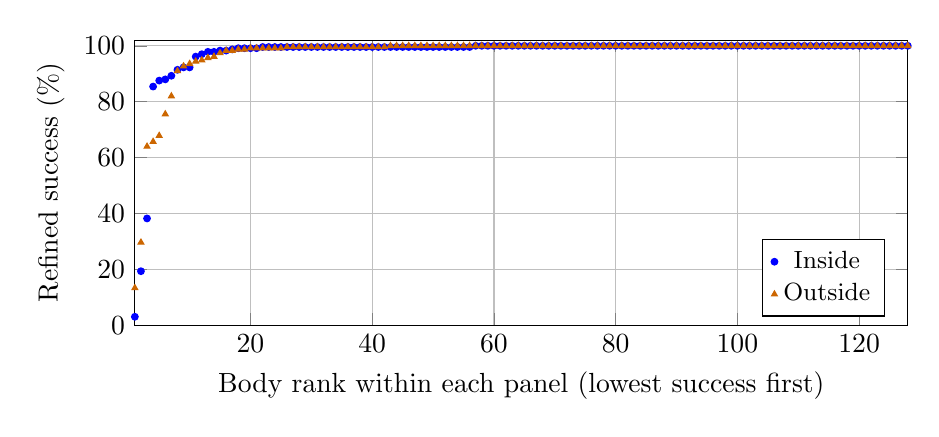
\begin{tikzpicture}
\begin{axis}[width=0.94\linewidth,height=5.2cm,
xlabel={Body rank within each panel (lowest success first)},
ylabel={Refined success (\%)},xmin=1,xmax=128,ymin=0,ymax=102,
legend pos=south east,legend style={font=\small},grid=major]

\addplot[only marks,mark=*,mark size=1.2pt,blue] coordinates {
(1,3.00) (2,19.31) (3,38.20) (4,85.41) (5,87.55) (6,87.98) (7,89.27) (8,91.42) (9,92.27) (10,92.27) (11,96.14) (12,97.00) (13,97.85) (14,97.85) (15,98.28) (16,98.28) (17,98.71) (18,99.14) (19,99.14) (20,99.14) (21,99.14) (22,99.57) (23,99.57) (24,99.57) (25,99.57) (26,99.57) (27,99.57) (28,99.57) (29,99.57) (30,99.57) (31,99.57) (32,99.57) (33,99.57) (34,99.57) (35,99.57) (36,99.57) (37,99.57) (38,99.57) (39,99.57) (40,99.57) (41,99.57) (42,99.57) (43,99.57) (44,99.57) (45,99.57) (46,99.57) (47,99.57) (48,99.57) (49,99.57) (50,99.57) (51,99.57) (52,99.57) (53,99.57) (54,99.57) (55,99.57) (56,99.57) (57,100.00) (58,100.00) (59,100.00) (60,100.00) (61,100.00) (62,100.00) (63,100.00) (64,100.00) (65,100.00) (66,100.00) (67,100.00) (68,100.00) (69,100.00) (70,100.00) (71,100.00) (72,100.00) (73,100.00) (74,100.00) (75,100.00) (76,100.00) (77,100.00) (78,100.00) (79,100.00) (80,100.00) (81,100.00) (82,100.00) (83,100.00) (84,100.00) (85,100.00) (86,100.00) (87,100.00) (88,100.00) (89,100.00) (90,100.00) (91,100.00) (92,100.00) (93,100.00) (94,100.00) (95,100.00) (96,100.00) (97,100.00) (98,100.00) (99,100.00) (100,100.00) (101,100.00) (102,100.00) (103,100.00) (104,100.00) (105,100.00) (106,100.00) (107,100.00) (108,100.00) (109,100.00) (110,100.00) (111,100.00) (112,100.00) (113,100.00) (114,100.00) (115,100.00) (116,100.00) (117,100.00) (118,100.00) (119,100.00) (120,100.00) (121,100.00) (122,100.00) (123,100.00) (124,100.00) (125,100.00) (126,100.00) (127,100.00) (128,100.00)
};\addlegendentry{Inside}
\addplot[only marks,mark=triangle*,mark size=1.2pt,orange!80!black] coordinates {
(1,13.30) (2,29.61) (3,63.95) (4,65.67) (5,67.81) (6,75.54) (7,81.97) (8,90.99) (9,92.70) (10,93.56) (11,94.42) (12,94.85) (13,95.71) (14,96.14) (15,97.42) (16,98.28) (17,98.28) (18,98.71) (19,98.71) (20,99.14) (21,99.14) (22,99.14) (23,99.14) (24,99.14) (25,99.14) (26,99.57) (27,99.57) (28,99.57) (29,99.57) (30,99.57) (31,99.57) (32,99.57) (33,99.57) (34,99.57) (35,99.57) (36,99.57) (37,99.57) (38,99.57) (39,99.57) (40,99.57) (41,99.57) (42,99.57) (43,100.00) (44,100.00) (45,100.00) (46,100.00) (47,100.00) (48,100.00) (49,100.00) (50,100.00) (51,100.00) (52,100.00) (53,100.00) (54,100.00) (55,100.00) (56,100.00) (57,100.00) (58,100.00) (59,100.00) (60,100.00) (61,100.00) (62,100.00) (63,100.00) (64,100.00) (65,100.00) (66,100.00) (67,100.00) (68,100.00) (69,100.00) (70,100.00) (71,100.00) (72,100.00) (73,100.00) (74,100.00) (75,100.00) (76,100.00) (77,100.00) (78,100.00) (79,100.00) (80,100.00) (81,100.00) (82,100.00) (83,100.00) (84,100.00) (85,100.00) (86,100.00) (87,100.00) (88,100.00) (89,100.00) (90,100.00) (91,100.00) (92,100.00) (93,100.00) (94,100.00) (95,100.00) (96,100.00) (97,100.00) (98,100.00) (99,100.00) (100,100.00) (101,100.00) (102,100.00) (103,100.00) (104,100.00) (105,100.00) (106,100.00) (107,100.00) (108,100.00) (109,100.00) (110,100.00) (111,100.00) (112,100.00) (113,100.00) (114,100.00) (115,100.00) (116,100.00) (117,100.00) (118,100.00) (119,100.00) (120,100.00) (121,100.00) (122,100.00) (123,100.00) (124,100.00) (125,100.00) (126,100.00) (127,100.00) (128,100.00)
};\addlegendentry{Outside}
\end{axis}\end{tikzpicture}
\caption{Unseen-body success, sorted within each panel.}\label{fig:unseen_v2_shapes}
\end{figure}

\paragraph{Checkpoint sensitivity.}
The later full-data checkpoint (epoch 34,000) was trained on all original motion
splits and differs from the original (epoch 28,170, distinct from the epoch-28,159
monitoring snapshot of Appendix~\ref{app:history}) by $-0.37$ pp inside and
$+0.42$ pp outside (Table~\ref{tab:unseen_v2}). Paired 95\% bootstrap intervals
resample clips with the body panel fixed, not training seeds or unseen bodies,
and a change counts as beyond noise only if its interval excludes zero and its
magnitude exceeds the identical-checkpoint rerun delta; both changes qualify,
but duration and motion coverage changed together, so they cannot be attributed
to either, and without a checkpoint ladder ordinary checkpoint variation remains
unmeasured. Identical-checkpoint reruns agree on 99.33\% of inside and 98.68\%
of outside pair labels (99.96\% in the control), yet individual pairs can change
by metres in peak error, so small pooled changes coexist with local instability.
The outside gain is concentrated in the ten bodies beyond the trained mass range
($+7.68$ pp, 95\% CI [$+6.39$, $+9.01$]) and the outermost coefficient tier
($+1.39$ pp [$+1.07$, $+1.72$]), while mean position error rises by 2.4, 5.0, and
3.1\,mm in the outside, inside, and control panels, so threshold success and
continuous tracking move differently. Three inside and six outside bodies regress
by more than 2 pp with intervals excluding zero, by up to 36.5 pp (per-body
intervals are exploratory and unadjusted for multiple testing), and five outside
bodies improve by more than 2 pp, including \texttt{male\_1c099619} (13.3\% to
71.2\%) (Appendix~\ref{app:unseen_tables}); neither improved extremes nor a
higher outside average justify calling the later checkpoint uniformly better. On
the 23-clip diagnostic subset, which the later checkpoint trained on, inside
success is 97.08\% versus 96.50\% and outside 96.81\% versus 96.91\% for the
original and later checkpoints; these values are excluded from the headline.
Severe failures remain unresolved: per-asset reference feasibility and
synchronized contact, root-height, and actuation traces have not been audited, so
reference, controller, and asset mechanisms cannot be distinguished.

\paragraph{Design comparisons.}\label{sec:design}
We compare four architectures: A, temporal MLP; B, temporal attention; C,
attention with slot/type embeddings, the architecture of MorphMimic; and D, C
with actor-only adaLN-Zero. All retain morphology inputs in actor and critic.
Refined-reference runs use three seeds (0, 1, 2) and a matched 6,000-epoch
budget on the development subset (Table~\ref{tab:architecture_seeds}), and each
run contributes one summary, the mean
of its last eight evaluations (epochs 4,600--6,000); means and sample standard
deviations are computed across the three run summaries, and within-run
evaluations are not replicates. Seed-1/2 values were checked against local
TensorBoard records, whereas the original logs of the seed-0 values were not
independently available. The full-scale MorphMimic model predates these reruns, which
reassess its design rather than establish prospective selection. Cases E--H
repeat A--D with unrefined references and one seed each
(Appendix~\ref{app:history}).

\begin{table}[t]
\centering\small
\caption{Three-seed refined-reference comparison, mean $\pm$ standard deviation across seeds.}\label{tab:architecture_seeds}
\begin{tabularx}{\linewidth}{@{}Yrrrrr@{}}
\toprule
Architecture & Success (\%) & Pos. (m) & Rot. (rad) & Jerk & Params (M) \\
\midrule
A: temporal MLP & $95.14\pm2.07$ & 0.118 & 0.216 & $2{,}110\pm643$ & 65.9 \\
B: temporal attention & $97.56\pm0.34$ & 0.090 & 0.218 & $2{,}783\pm887$ & 51.2 \\
C: slot/type attention & $97.89\pm0.22$ & 0.090 & 0.219 & $2{,}413\pm762$ & 51.2 \\
D: C + adaLN-Zero & $97.17\pm0.08$ & 0.083 & 0.211 & $2{,}659\pm674$ & 52.1 \\
\bottomrule
\end{tabularx}
\end{table}

Position and rotation errors are across-seed means, and parameters are actor
and critic totals. Attention variants reach 97.2--97.9\% mean success against
95.1\% for the temporal MLP, with lower position error (0.083--0.090 versus
0.118\,m) and much smaller seed variability (standard deviation 0.08--0.34
versus 2.07 points), although the MLP has the most parameters, roughly
26--29\% more than the attention variants. Among the attention variants, C has
the highest mean success and D the lowest position and rotation errors. A has
the lowest mean jerk, but jerk differences between architectures are
comparable to the seed-to-seed standard deviations (643--887), so the apparent
factor-of-two jerk advantage in seed 0 is not a consistent architecture
effect. Three seeds do not establish statistical superiority, and MorphMimic
uses C as a practical compromise.

\paragraph{Reference refinement.}\label{sec:refinement_results}
A paired offline audit of all 19,200 development references (150 clips
$\times$ 128 bodies; no simulation) compares artifact and fidelity measures
before and after refinement (Table~\ref{tab:refine_audit}). Artifact rows give
the corpus mean before and after and the fraction of motions that improve;
fidelity rows give the corpus mean refined-versus-unrefined difference.
Refinement lowers stance-foot speed during detected contact from 0.055 to
0.038\,m/s, with 96\% of references improving, and below-floor frames from
39.6\% to 3.3\% (only 45\% of references improve on the latter because many
were already grounded). Measured motion features are largely preserved: the mean
per-body rotation change is $0.12^\circ$, root horizontal displacement is
0.008\,m, and the cross-shape variance of knee-flexion range is retained at a
ratio of 0.94. The cost is higher reference jerk (the raw mean third difference
of body positions, not the windowed evaluator score), from 45.2 to
60.7\,m/s$^3$, with 79\% of references worsening; temporal root and clearance
corrections are a candidate explanation, but their contribution to policy
smoothness is not isolated. Refined and unrefined policies (cases A--D versus
E--H) track different targets, so their comparison describes different tasks
and does not establish a causal benefit of refinement, which would need a
common-reference checkpoint comparison.

\begin{table}[!htb]
\centering
\small
\caption{Reference-refinement audit over 19,200 development references.}\label{tab:refine_audit}
\begin{tabularx}{\linewidth}{@{}Yrrr@{}}
\toprule
& Unref.\ mean & Refined mean & Motions improved \\
\midrule
Stance-foot speed (m/s) $\downarrow$ & 0.055 & 0.038 & 96\% \\
Frames below floor (\%) $\downarrow$ & 39.6 & 3.3 & 45\% \\
Frames within 2\,cm of floor (\%) $\downarrow$ & 49.8 & 33.6 & --- \\
Position jerk (m/s$^3$) & 45.2 & 60.7 & 21\% \\
\midrule
Per-body rotation change (deg) & \multicolumn{3}{c}{0.12} \\
Root horizontal displacement (m) & \multicolumn{3}{c}{0.008} \\
Cross-shape var., knee-flexion range (ratio r/u) & \multicolumn{3}{c}{0.94} \\
\bottomrule
\end{tabularx}
\end{table}

\paragraph{Scope of the morphology-conditioning evidence.}
Every architecture receives morphology inputs in actor and critic. The adaLN-Zero
variant changes how the actor uses them but does not test their removal, and
body-dependent state and reference targets also expose morphology. Successful
transfer therefore establishes a capability of the whole system, not that
explicit coefficients cause it. Attributing it to those inputs needs a matched
training run without them, with the same references, body panel, budget, and
seeds; inference-time masking or shuffling would introduce distribution shift
and cannot replace that comparison.
